\documentclass[a11paper]{article}

\usepackage{karnaugh-map}
\usepackage{subcaption}
\usepackage{tabularx}
\usepackage{titlepage}
\usepackage{document}
\usepackage{tools}
\usepackage{booktabs}
\usepackage{multicol}
\usepackage{multirow}
\usepackage{float}
\usepackage{longtable}
\usepackage{varwidth}
\usepackage{graphicx}
\usepackage{siunitx}
\usepackage{pifont}
\usepackage{tikz}
\usetikzlibrary{automata, positioning, arrows}
% \usepackage[toc,page]{appendix}
\usepackage[usenames,dvipsnames]{xcolor}

\title{Rapport d'APP}

\class{Éléments de compilation}
\classnb{GIF340}

\teacher{Marouane Adnane}

\author{
  \addtolength{\tabcolsep}{-0.4em}
  \begin{tabular}{rcl} % Ajouter des auteurs au besoin
      Benjamin Chausse & -- & CHAB1704 \\
      Shawn Couture    & -- & COUS1912 \\
  \end{tabular}
}


\renewcommand{\frenchtablename}{Tableau}


\begin{document}
\maketitle
\newpage
\tableofcontents
\listoffigures
\listoftables

\newpage

\section{Définition des unités lexicales}
\todo{Décrire formellement des unités lexicales à l’aide d’expressions
régulières et d’automates à états
finis.}\\

\section{Description de la grammaire}
\todo{Décrire formellement une syntaxe à l’aide d’une grammaire.} \\

\todo{Analyser et manipuler une grammaire.} \\

\section{Analyseur lexical}
\todo{Concevoir et réaliser un analyseur lexical.} \\

\section{Analyseur syntaxique}
\todo{Concevoir et réaliser un analyseur syntaxique.} \\


\appendix

\section{Machines à état finie}

\begin{figure}[H]
\centering
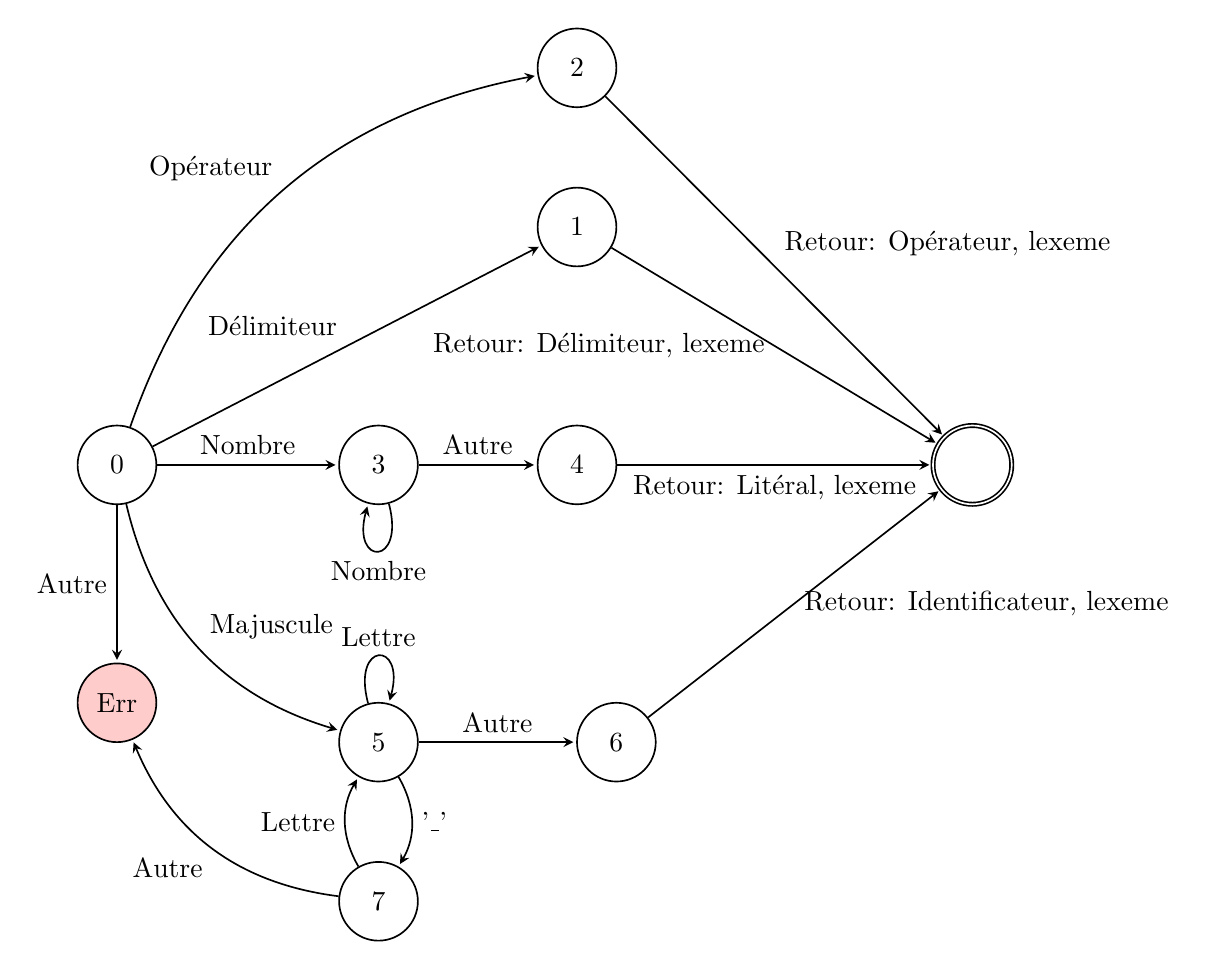
\begin{tikzpicture}[
    > = stealth,
    shorten > = 1pt,
    auto,
    node distance = 2cm,
    semithick,
    state/.style = {circle, draw, minimum size = 1cm},
    error/.style = {circle, draw, fill = red!20, minimum size = 1cm},
    final/.style = {circle, draw, double, minimum size = 1cm}
]

% States
\node[state]                     (0)     {0};
\node[state, right = 2.3cm of 0] (3)     {3};
\node[state, right = 1.5cm of 3] (4)     {4};
\node[state, above = of 4]       (1)     {1};
\node[state, above = 1cm of 1]   (2)     {2};
\node[state, below = 2.5cm of 3] (5)     {5};
\node[state, below = 1cm of 5]   (7)     {7};
\node[state, right = of 5]       (6)     {6};
\node[error, below = of 0]       (err)   {Err};
\node[final, right = 4cm of 4]   (final) {};

\draw[->] (0) to             node[left] {Autre}      (err);
\draw[->] (0) to             node       {Délimiteur} (1);
\draw[->] (0) to             node       {Nombre}     (3);
\draw[->] (0) to[bend left]  node       {Opérateur}  (2);
\draw[->] (0) to[bend right] node       {Majuscule}  (5);

\draw[->] (1) to node[left] {Retour: Délimiteur, lexeme} (final);

\draw[->] (2) to node {Retour: Opérateur, lexeme} (final);

\draw[->] (3) to[loop below] node {Nombre} (3);
\draw[->] (3) to             node {Autre}  (4);

\draw[->] (4) to node[below] {Retour: Litéral, lexeme} (final);

\draw[->] (5) to[loop above] node {Lettre} (5);
\draw[->] (5) to             node {Autre}  (6);
\draw[->] (5) to[bend left]  node {'\_'}   (7);

\draw[->] (6) to node[right] {Retour: Identificateur, lexeme} (final);

\draw[->] (7) to[bend left] node {Lettre} (5);
\draw[->] (7) to[bend left] node {Autre}  (err);

\end{tikzpicture}

\caption{Mise en unités lexicales}
\end{figure}

% \begin{figure}[H]
% \centering
% 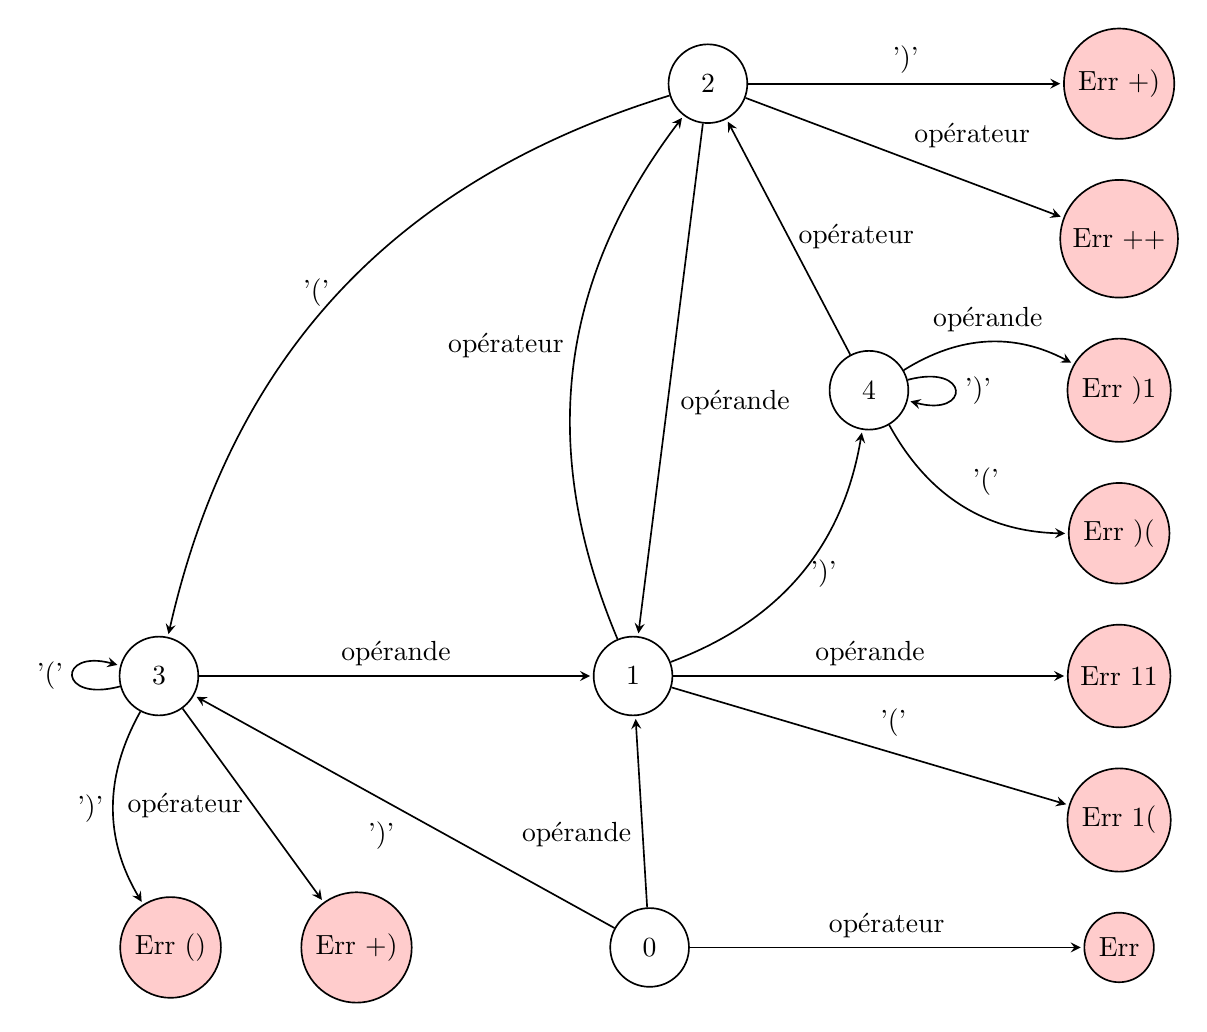
\begin{tikzpicture}[
    > = stealth,
    shorten > = 1pt,
    auto,
    node distance = 2cm,
    semithick,
    state/.style = {circle, draw, minimum size = 1cm},
    error/.style = {circle, draw, fill = red!20, minimum size = .5cm},
    final/.style = {circle, draw, double, minimum size = 1cm}
]

% States
\node[error]                            (err)       {Err};
\node[error, above = .5cm of err]       (errIntPar) {Err 1(};
\node[error, above = .5cm of errIntPar] (errIntInt) {Err 11};
\node[error, above = .5cm of errIntInt] (errParPar) {Err )(};
\node[error, above = .5cm of errParPar] (errParInt) {Err )1};
\node[error, above = .5cm of errParInt] (errOpOp)   {Err ++};
\node[error, above = .5cm of errOpOp]   (errOpPar)  {Err +)};

\node[state, left = 5cm of err]       (0) {0};
\node[state, left = 5cm of errIntInt] (1) {1};
\node[state, left = 5cm of 1]         (3) {3};
\node[state, left = 4cm of errOpPar]  (2) {2};
\node[state, left = 2cm of errParInt] (4) {4};

\node[error, left = 2.5cm of 0]      (errParOp) {Err +)};
\node[error, left = 1cm of errParOp] (errEmpty) {Err ()};


% Transitions from state 0
\draw[->] (0) to            node {opérateur} (err);
\draw[->] (0) to            node {opérande}  (1);
\draw[->] (0) to node {')'}       (3);

\draw[->] (1) to[bend left] node {opérateur} (2);
\draw[->] (1) to[bend right] node[right] {')'}       (4);
\draw[->] (1) to            node {'('}       (errIntPar);
\draw[->] (1) to            node {opérande}  (errIntInt);

\draw[->] (2) to[bend right] node[left] {'('}       (3);
\draw[->] (2) to             node       {opérande}  (1);
\draw[->] (2) to             node       {opérateur} (errOpOp);
\draw[->] (2) to             node       {')'}       (errOpPar);

\draw[->] (3) to[loop left]  node       {'('}       (3);
\draw[->] (3) to             node[left] {opérateur} (errParOp);
\draw[->] (3) to[bend right] node[left] {')'}       (errEmpty);
\draw[->] (3) to node                   {opérande}  (1);

\draw[->] (4) to             node[right] {opérateur} (2);
\draw[->] (4) to[loop right] node        {')'}       (4);
\draw[->] (4) to[bend right] node        {'('}       (errParPar);
\draw[->] (4) to[bend left]  node        {opérande}  (errParInt);

\end{tikzpicture}

% \caption{Analyse lexicale}
% \end{figure}

\quickfig{MEF de détection d'un délimiteur}{fsm-delimiter}{.7}{assets/img/fsm-delimiter.png}
\quickfig{MEF de détection d'un identificateur}{fsm-identifier}{.7}{assets/img/fsm-identifier.png}
\quickfig{MEF de détection d'un litéral}{fsm-literal}{.7}{assets/img/fsm-literal.png}
\quickfig{MEF de détection d'un opérateur}{fsm-operator}{.7}{assets/img/fsm-operator.png}

\newpage
\section{Arbres syntaxiques}

\quickfig{Représentation graphique du json généré par le test \#\ref{tid:first}}{ast-first}{.85}{assets/img/ast-1.png}
\quickfig{Représentation graphique du json généré si le test \#\ref{tid:first} n'avait pas de parenthèses}{ast-err}{.85}{assets/img/ast-err.png}
% \quickfig{Représentation graphique du json généré par le test \#\ref{tid:second}}{ast-second}{.85}{assets/img/ast-2.png}
\quickfig{Représentation graphique du json généré par le test \#\ref{tid:sum}}{ast-sum}{.6}{assets/img/ast-E.png}
\quickfig{Représentation graphique du json généré par le test \#\ref{tid:prod}}{ast-prod}{.6}{assets/img/ast-T.png}

\newpage
\section{Messages d'erreurs}

\begin{error}[Message d'erreur issu du test \#\ref{tid:start-op}]{err:start-op}
\begin{verbatim}
app6.SyntaxException: Syntax Error at position 0: Unexpected token
  Expected: literal, identifier, or '('
  Found: +
  Context: +2-3
\end{verbatim}
\end{error}

\begin{error}[Message d'erreur issu du test \#\ref{tid:end-op}]{err:end-op}
\begin{verbatim}
app6.SyntaxException: Syntax Error at position 3: Expected operand after operator
  Expected: number or expression
  Found: end of input
  Context: *
\end{verbatim}
\end{error}

\begin{error}[Message d'erreur issu du test \#\ref{tid:double-op}]{err:double-op}
\begin{verbatim}
app6.SyntaxException: Syntax Error at position 2: Unexpected token
  Expected: literal, identifier, or '('
  Found: /
  Context: /2-3
\end{verbatim}
\end{error}

\begin{error}[Message d'erreur issu du test \#\ref{tid:missing-close}]{err:missing-close}
\begin{verbatim}
app6.SyntaxException: Syntax Error at position 6: Expected closing parenthesis
  Expected: ')'
  Found: end of input
\end{verbatim}
\end{error}

\begin{error}[Message d'erreur issu du test \#\ref{tid:missing-open}]{err:missing-open}
\begin{verbatim}
app6.SyntaxException: Syntax Error at position 3: Failed to parse complete
expression - unexpected tokens remain
  Found: )
  Context: ) - 3
\end{verbatim}
\end{error}

\begin{error}[Message d'erreur issu du test \#\ref{tid:empty-paren}]{err:empty-paren}
\begin{verbatim}
app6.SyntaxException: Syntax Error at position 5: Expected opening parenthesis
  Expected: '('
  Found: )
  Context: )/3
\end{verbatim}
\end{error}





\end{document}
